\section{Descriptive Data Analysis}

\subsection{Types of Variables}

One of the first stages of descriptive analysis is to recognize the different types of data, as these observations are a representation of the world around us through what are called variables. A variable is a characteristic or attribute of an object that can be observed and measured, assuming different values. Variables can be represented in different forms: numerical (discrete and continuous) or categorical (nominal and ordinal). Figure~\ref{fig:variable_types} summarizes the classification of variable types.

\begin{figure}[H]
\centering
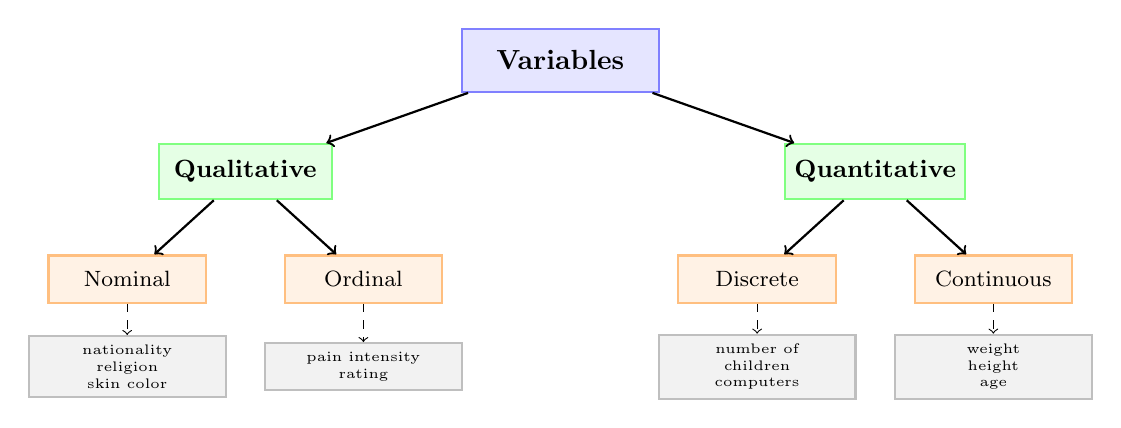
\begin{tikzpicture}[
    every node/.style={align=center},
    root/.style={rectangle, draw=blue!50, fill=blue!10, thick, minimum width=2.5cm, minimum height=0.8cm, font=\bfseries},
    main/.style={rectangle, draw=green!50, fill=green!10, thick, minimum width=2.2cm, minimum height=0.7cm, font=\small\bfseries},
    leaf/.style={rectangle, draw=orange!50, fill=orange!10, thick, minimum width=2cm, minimum height=0.6cm, font=\footnotesize},
    example/.style={rectangle, draw=gray!50, fill=gray!10, thick, minimum width=2.5cm, minimum height=0.5cm, font=\tiny, text width=2.2cm}
]
    % Root node
    \node[root] (variables) at (0,0) {Variables};
    
    % Main branches
    \node[main] (qualitative) at ([xshift=-4cm, yshift=-1cm]variables.south) {Qualitative};
    \node[main] (quantitative) at ([xshift=4cm, yshift=-1cm]variables.south) {Quantitative};
    
    % Qualitative subtypes
    \node[leaf] (nominal) at ([xshift=-1.5cm, yshift=-1cm]qualitative.south) {Nominal};
    \node[leaf] (ordinal) at ([xshift=1.5cm, yshift=-1cm]qualitative.south) {Ordinal};
    
    % Quantitative subtypes
    \node[leaf] (discrete) at ([xshift=-1.5cm, yshift=-1cm]quantitative.south) {Discrete};
    \node[leaf] (continuous) at ([xshift=1.5cm, yshift=-1cm]quantitative.south) {Continuous};
    
    % Example boxes
    \node[example] (nominal_ex) at ([yshift=-0.8cm]nominal.south) {nationality\\religion\\skin color};
    \node[example] (ordinal_ex) at ([yshift=-0.8cm]ordinal.south) {pain intensity\\rating};
    \node[example] (discrete_ex) at ([yshift=-0.8cm]discrete.south) {number of\\children\\computers};
    \node[example] (continuous_ex) at ([yshift=-0.8cm]continuous.south) {weight\\height\\age};
    
    % Connections
    \draw[->, thick] (variables) -- (qualitative);
    \draw[->, thick] (variables) -- (quantitative);
    \draw[->, thick] (qualitative) -- (nominal);
    \draw[->, thick] (qualitative) -- (ordinal);
    \draw[->, thick] (quantitative) -- (discrete);
    \draw[->, thick] (quantitative) -- (continuous);
    \draw[->, thin, dashed] (nominal) -- (nominal_ex);
    \draw[->, thin, dashed] (ordinal) -- (ordinal_ex);
    \draw[->, thin, dashed] (discrete) -- (discrete_ex);
    \draw[->, thin, dashed] (continuous) -- (continuous_ex);
\end{tikzpicture}
\caption{Classification of variable types}
\label{fig:variable_types}
\end{figure}

\subsubsection{Qualitative Variable}

A qualitative variable expresses a characteristic in a non-numerical form, representing a quality. Examples: color, gender, blood type, marital status. It can be of two types:

\begin{itemize}
    \item \textbf{Nominal:} Values are codes or names that cannot be ordered. Examples: nationality, religion, skin color.
    
    \item \textbf{Ordinal:} Values imply an ordering from greater to lesser or from better to worse. Examples: pain intensity (absent, mild, moderate, severe, very severe), rating (excellent, good, fair, poor).
\end{itemize}

\subsubsection{Quantitative Variable}

A quantitative variable is expressed by means of a number. It can be of two types:

\begin{itemize}
    \item \textbf{Discrete:} Only admits a finite set of numerical values, usually integers. Examples: number of children per household, number of computers in a classroom, number of electrons in an atom.
    
    \item \textbf{Continuous:} Can take infinitely many possible values within a range or interval on the real number line. These variables represent measurements whose values cannot be enumerated. Examples: weight (kg), height, age, the time it takes an athlete to run 100 meters.
\end{itemize}

\subsection{Characterization of Variable Distributions}

\subsubsection{Histogram}

A histogram is a graphical representation of the distribution of numerical data. It displays the frequency of data points within specified intervals (bins). The x-axis represents the intervals, and the y-axis represents the frequency or relative frequency. The bars are adjacent to each other, unlike bar charts for categorical data.

Histograms are used for continuous or discrete quantitative variables. The bin width affects the appearance and interpretation. The area of each bar is proportional to the frequency, with no gaps between bars (unless a bin has zero frequency). Histograms reveal the shape, center, and spread of the data distribution.

To read a histogram, examine the overall shape (symmetric, skewed, or multimodal), identify the center, assess the spread, and look for outliers or unusual patterns.

Figure~\ref{fig:histogram_example} shows an example of a histogram. Its shape depends on the number of intervals, and the symmetry can vary; the more similar the values on both sides of the center, the more symmetric the distribution (Rodríguez Ojeda, 2007):

\begin{itemize}
    \item If the height or y-axis of the bars are similar to each other, we would have a uniform distribution.
    
    \item If the heights are greater in the central zone, a ``bell'' shape is formed, which can be symmetric or asymmetric, toward the positive side (to the right) or negative (to the left).
    
    \item If there are bars far from the group, they are considered atypical data, which are probably due to measurement errors and can be discarded, as they do not belong to the group that is desired to be characterized (Rodríguez Ojeda, 2007).
\end{itemize}

\begin{figure}[H]
\centering
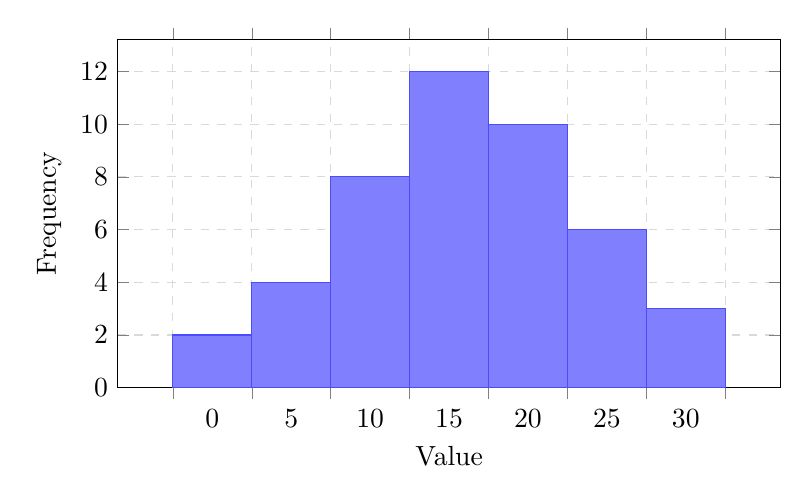
\begin{tikzpicture}
\begin{axis}[
    ybar interval,
    ymin=0,
    xlabel={Value},
    ylabel={Frequency},
    width=10cm,
    height=6cm,
    bar width=0.8,
    xtick={0,5,10,15,20,25,30,35,40},
    xticklabels={0,5,10,15,20,25,30,35,40},
    ytick={0,2,4,6,8,10,12},
    grid=major,
    grid style={dashed, gray!30}
]
\addplot[fill=blue!50, draw=blue!70] coordinates {
    (0,2) (5,4) (10,8) (15,12) (20,10) (25,6) (30,3) (35,1)
};
\end{axis}
\end{tikzpicture}
\caption{Example of a histogram showing a bell-shaped distribution}
\label{fig:histogram_example}
\end{figure}

